\section{Sidebar: Outcome diagram and plots}

    \subsection{Creating the system/outcome diagrams}

    You need to provide a textual description of your outcome diagram following the syntax which was defined previously (\cref{out_syntax}).
    You can create your system by clicking on the \textbf{Create or edit system} button (\cref{fig:savsys}). If the parser successfully parsed the text, your system will be created, and you can start setting the parameters for your probes.
    
    \begin{figure}[H]
        \begin{center}
            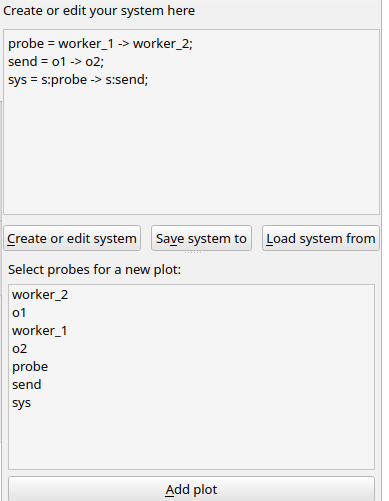
\includegraphics[width = \textwidth]{img/manual/after_create.png}
        \end{center}
        \caption{After selecting create system, if the system definition is correct, the inserted probes will be available to be plotted.}
        \label{fig:savsys}
    \end{figure}

    If the parser does not correctly parse the text, it will show a popup indicating the line where the error was produced and what it was expecting (\cref{fig:syserr}). If there is a cycle, it will specify where it found the cycle.  
     
    \begin{figure}[H]
        \begin{center}
            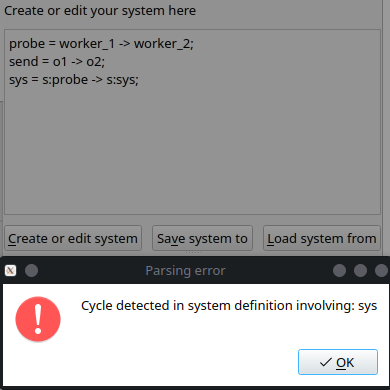
\includegraphics[width = \textwidth]{img/manual/cycle.png}
        \end{center}
        \caption{Creation of a system with a cycle}
        \label{fig:syserr}
    \end{figure}


    \subsection{Saving the system definition}

    The button \textbf{Save system to} gives you the possibility to save the textual definition of the outcome diagram to a file. You can save the file to any extension, but preferably the file will have the \textbf{.dq} extension (\cref{fig:loadsys}).

    \subsection{Loading the system definition}

    The button \textbf{Load system to} gives you the possibility to load the textual definition of the outcome diagram you may have previously saved to a file (\cref{fig:loadsys}). As for the extension, you can load any file extension.

    
    \begin{figure}[H]
        \begin{center}
            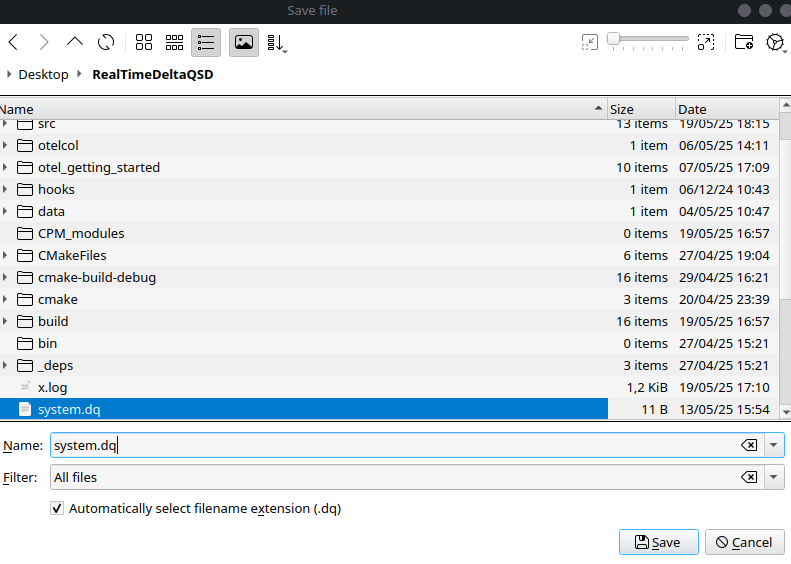
\includegraphics[width = \textwidth]{img/save_system.png}
        \end{center}
        \caption{Example popup where the user can select a file where the system definition is loaded.}
        \label{fig:loadsys}
    \end{figure}
        
\subsection{Changing the sampling rate}
    The user can set the sampling rate via the slider in this tab (\cref{fig:slid_wid}):
 \begin{figure}[H]
        \begin{center}
            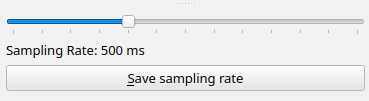
\includegraphics[width = \textwidth]{img/manual/modify_sampling.png}
        \end{center}
        \caption{Slider widget.}
        \label{fig:slid_wid}
    \end{figure}

\subsection{Managing the plots} 
    Once you have your system defined you can start adding plots of the $\Delta$Qs of the probes you inserted in your system.
    
    \subsubsection{Adding a plot}

    Multiple probes can be added at once in your plot, you can select the probes you want to add to a new plot by selecting them in the \textbf{``Add a new plot''} section (\cref{fig:sel_prob}). Then by clicking the \textbf{``Add plot''} button, the selected probes will be added to the plot (\cref{fig:new_sel}). 
 
    \begin{figure}[H]
        \begin{center}
        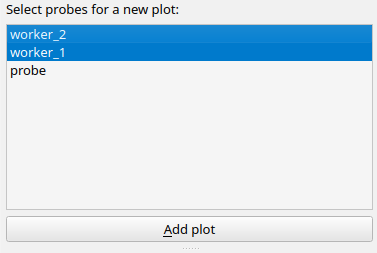
\includegraphics[width = \textwidth]{img/manual/add_plot2.png}
        \end{center}
        \caption{Selecting the probes to add to a plot}
        \label{fig:sel_prob}
    \end{figure}

    \begin{figure}[H]
        \begin{center}
        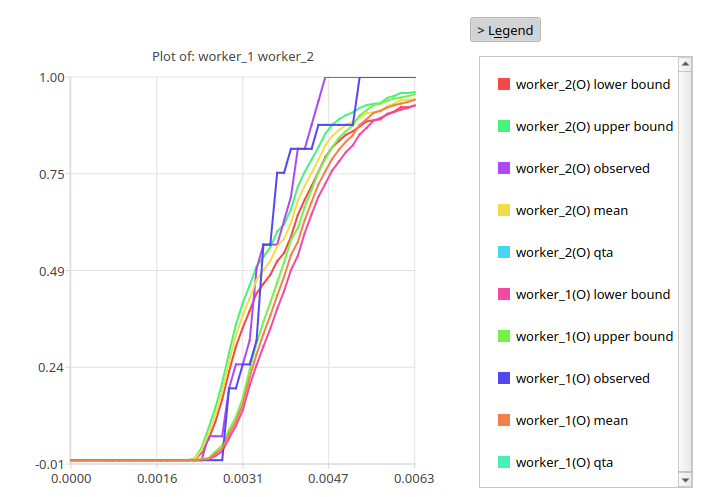
\includegraphics[width = \textwidth]{img/manual/running.png}
        \end{center}
        \caption{After adding the probe's to a plot, if the adapter is already sending spans, the plot will show the real time $\Delta$Qs.}
        \label{fig:new_sel}
    \end{figure}

\subsubsection{Editing a plot}
    You can remove the probes you have added to the plot by first clicking to it, this sets the plot as the \textbf{selected plot}. Once you have clicked the plot, a section will pop up beneath the rest of the controls on the sidebar. 
        

    In the section there are two subsections, one which shows the selected components which form the plot (those you have added previously), and the available components. You can select the probes you want to remove in the \textbf{``selected probes''} zone, by clicking \textbf{"Remove selected probes"} the components will be removed from the plot. Inversely, in the \textbf{``Available probes''} section, you can select the plots you want to add, and by clicking \textbf{"Add selected probes"} you can add the selected components to the selected plot (\cref{fig:edit_pl}).

        \begin{figure}[H]
            \centering
            \begin{subfigure}{.5\textwidth}
                \centering
                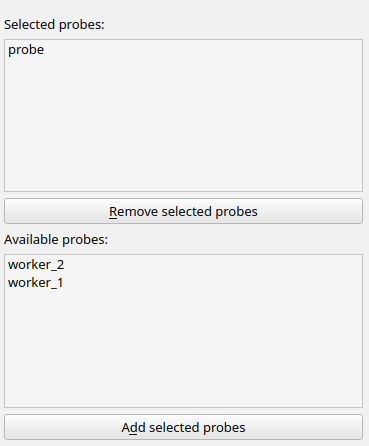
\includegraphics[width=0.98\textwidth]{img/manual/modify_plot.png}
            \end{subfigure}%
            \begin{subfigure}{.5\textwidth}
                \centering
                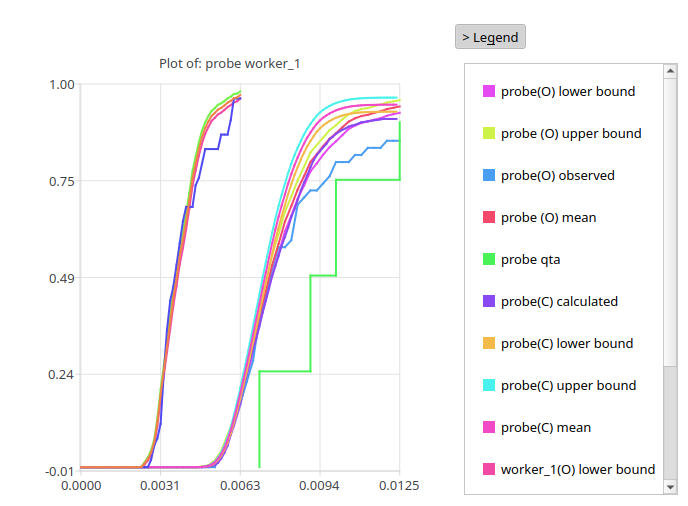
\includegraphics[width =0.98\textwidth]{img/manual/added_plot.png}
            \end{subfigure}
            \caption{To modify a plot, click on the probe you want to remove or add. Here, for example, worker\_1's probe was added by selecting it below and clicking "Add selected probes".}
            \label{fig:edit_pl}
        \end{figure}

\subsection{Removing a plot}
    By left-clicking the plot, a popup appears, you can click \textbf{"Remove plot"}, this removes it from the selected plot (\cref{fig:edit_pl}).
